\documentclass [xcolor=svgnames, t] {beamer}
\usepackage{graphicx}
\usepackage{tikz}
\usetikzlibrary{arrows.meta}
\tikzset{%
  >={Latex[width=2mm,length=2mm]},
  % Specifications for style of nodes:
            base/.style = {rectangle, rounded corners, draw=black,
                           minimum width=4cm, minimum height=1cm,
                           text centered, font=\sffamily},
  activityStarts/.style = {base, fill=blue!30},
       startstop/.style = {base, fill=red!30},
    activityRuns/.style = {base, fill=green!30},
         process/.style = {base, minimum width=2.5cm, fill=orange!15,
                           font=\ttfamily},
}

\usepackage[utf8]{inputenc}
\usepackage{booktabs, comment}
\usepackage[portuguese]{babel}
\usepackage[absolute, overlay]{textpos}
\usepackage{pgfpages}
\usepackage[font=footnotesize]{caption}
\useoutertheme{infolines}

\definecolor{brownbrown}{RGB}{56, 28, 0}
\definecolor{brownred}{RGB}{255, 0, 43}

\AtBeginSection[]{
  \begin{frame}
  \vfill
  \centering
  \begin{beamercolorbox}[sep=8pt,center,shadow=true,rounded=true]{title}
    \usebeamerfont{title}\insertsectionhead\par%
  \end{beamercolorbox}
  \vfill
  \end{frame}
}


\setbeamercolor{title in head/foot}{bg=brownred, fg=brownbrown}
\setbeamercolor{author in head/foot}{bg=myuniversity}
\setbeamertemplate{page number in head/foot}{}
\usepackage{csquotes}

\usepackage{amsmath}
\usepackage[makeroom]{cancel}

\usepackage{textpos}

\usetheme{Madrid}
\definecolor{myuniversity}{RGB}{0, 0, 0}
\usecolortheme[named=myuniversity]{structure}
\usepackage{tikz}

\title[Trabalho de Conclusão de Curso]{\textbf{Uma abordagem de sistemas
lineares a teoria de séries temporais estacionárias e não estacionárias}}
\subtitle{Apresentação de Trabalho de Conclusão de Curso}
\institute[]{Curso de Graduação em Engenharia Elétrica}

\titlegraphic{\includegraphics[height=2.0cm]{brown-logo.png}}

\author[Gabriel Lara]{ Gabriel Teixeira Lara Chaves }

\institute[]{Curso de Graduação em Engenharia Elétrica \\ Universidade Federal de Minas Gerais}

\addtobeamertemplate{navigation symbols}{}{%
    \usebeamerfont{footline}%
    \usebeamercolor[fg]{footline}%
    \hspace{1em}%
    \insertframenumber/\inserttotalframenumber
}

\begin{document}

\begin{frame}
\maketitle
\end{frame}

%%%%%%%%%%%%%%%%%%%%%%%%%%%%
\logo{\includegraphics[height=1.0cm]{brown-arms.png}~%
}
%%%%%%%%%%%%%%%%%%%%%%%%%%

\section{Contextualização}

\begin{frame}{Conteúdo}

\tableofcontents

\end{frame}

\section{Definições}

\begin{frame}{O que é uma série temporal?}

Uma série temporal é um conjunto de observações realizadas sequencialmente no
tempo, indexadas de acordo com o momento em que foram observadas. As
observações representam a realização de um processo estocástico.

$${\mathbf{y}}_{t=-\infty}^{\infty} = ({\dots, y_{-1},y_0, \overbrace{y_1, y_2, y_3, \dots, y_T}^{\text{Série Observada}}, y_{T+1}, y_{T+2}}\dots)$$

\vspace{.5cm}

O presente estudo aborda uma perspectiva de sistemas lineares para representar
processos estocásticos a partir de séries temporais estacionarias.

\end{frame}

\begin{frame}{Autocorrelação}

A função de autocorrelação é uma medida de semelhança de uma série com suas
amostras passadas, definida como a correlação entre um sinal e suas versões
sucessivamente atrasadas. A figura~\ref{fig:arcorr} ilustra alguns exemplos
de autocorrelações de sinais estacionários.

\begin{figure}[H]
\centering
\includegraphics[scale=0.3]{../figures/ar_corr.png}
\caption{Visualização de autocorrelação de processes autoregressivos
    de diferentes ordens.}
\label{fig:arcorr}
\end{figure}


\end{frame}

\begin{frame}{Estacionariedade}

Certas características de dados tabulares facilitam a inferência de
propriedades da função geradora a partir de observações, como
independência. Amostras de séries temporais são, de forma geral, dependentes.

\vspace{.5cm}

Estacionariedade é uma estrutura de dependência que permite o uso da Lei dos
Grandes Números, por exemplo, para estimar a distribuição subjacente.

\vspace{.5cm}

Sua versão mais restrita assume que a distribuição da série ao longo do tempo
é constante.


\end{frame}

\begin{frame}{Estacionariedade}

A visualização de autocorrelações invariantes ao tempo de sinais não
estacionários não fazem sentido porque sob essa condição a autocorrelação
é uma função do tempo de atraso. A figura~\ref{fig:trend_acorr} ilustra uma
autocorrelação típica de um sinal com tendência.

\begin{figure}[H]
    \centering
    \includegraphics[scale=0.3]{../figures/corr_trend.png}
    \caption{Autocorrelação de série com tendência.}
    \label{fig:trend_acorr}
\end{figure}

\end{frame}

\section{Modelos Lineares}

\begin{frame}{Modelo ARMA}

O modelo ARMA é definido pela equação de recorrência~\ref{eq:arma_l}, onde
amostras da série são modeladas como uma combinação linear de amostras
passadas da própria série e um sinal de ruído branco.

\vspace{0.5cm}

\begin{equation}\label{eq:arma_l}
    y_t = \varepsilon_t \frac{\phi(L)}{\theta(L)}
\end{equation}

\vspace{0.5cm}

Um processo $ARMA(2, 1)$ é portanto dado pela seguinte equação de recorrência.

$$ y_t = \alpha_1 y_{t-1} + \alpha_2 y_{t-2} + \varepsilon_{t} + \beta_1 \varepsilon_{t-1} $$

\end{frame}

\begin{frame}{Teorema de Wold}

Por expansão do fator polinomial $\frac{\phi(L)}{\theta(L)}$ concluímos que
qualquer modelo ARMA pode ser representado como regressão em atrasos
infinitamente longos de ruído branco. Eis o Teorema de Wold: qualquer sinal
estacionário possui representação da forma dada pela equação~\ref{eq:glm}.

\vspace{5mm}

\begin{equation}\label{eq:glm}
    y_t = \psi(L)\varepsilon_t = \sum^{\infty}_{0} \psi_m \varepsilon_t
\end{equation}

\vspace{5mm}

Esta forma de modelos ARMA é denominada um modelo linear generalizado.


\end{frame}

\begin{frame}{Modelos ARMA como filtros lineares}

Notamos imediatamente que qualquer sinal ARMA é, na verdade, o resultado da
filtragem IIR de ruído branco.

\vspace{5mm}

\begin{figure}
    \centering
    \begin{tikzpicture}[node distance=4.5cm,
        every node/.style={fill=white, font=\sffamily}, align=center]

        \node (system)      [activityStarts]              {Sistema LTI\\$\psi(t)$};
        \node (input)       [process, left of=system]     {$\varepsilon_t$};
        \node (output)      [process, right of=system]    {$y_t$};

        \draw[->]     (input) -- (system);
        \draw[->]     (system) -- (output);

    \end{tikzpicture}
    \vspace{.6cm}
    \caption{Representação de série temporal como modelo linear generalizado}
    \label{fig:white_noise_LTI}
\end{figure}

Essa compreensão do processo gerador de uma série temporal estacionária
naturalmente define quase toda a teoria de séries temporais em função de
ideias de sistemas lineares: estacionariedade, invertibilidade, raízes
unitárias, etc...

\end{frame}

\begin{frame}{Modelos ARMA como filtros lineares}

Concluímos então que uma série temporal gerada por um processo $AR(p)$
corresponde a um filtro IIR e uma gerada por um processo $MA(q)$ a um filtro
FIR.

\vspace{5mm}

Uma série é estacionária se seu polinômio autoregressivo possuir raízes,
em $L$, fora do círculo unitário. É inversível se seu polinômio média móvel
possuir raízes na mesma posição.

\vspace{5mm}

É possível traçar paralelos entre conceitos de sistemas lineares e séries
temporais sobre essa ótica.

\end{frame}

\begin{frame}{Modelos ARMA como filtros lineares}


    \begin{figure}[H]
        \centering
        \includegraphics[scale=0.5]{../figures/arma_21_pzp.png}
    \end{figure}

\end{frame}


\begin{frame}{Modelos ARMA como filtros lineares}

\vspace{5mm}

\begin{table}[H]
\centering
\begin{tabular}{|l|l|}
\hline
\textbf{Séries Temporais} & \textbf{Processamento de Sinais} \\ \hline
Estacionariedade          & Estabilidade                     \\ \hline
Invertibilidade           & Invertibilidade                  \\ \hline
Raíz Unitária             & Estabilidade Marginal            \\ \hline
AR                        & Filtro IIR                       \\ \hline
MA                        & Filtro FIR                       \\ \hline
\end{tabular}
\end{table}

\end{frame}

\begin{frame}{Modelos ARMA como filtros lineares}

\hspace{1cm}Quais os limites dessa comunicação?

\begin{figure}[!tbp]
  \centering
  \begin{minipage}[b]{0.4\textwidth}
    
\includegraphics[width=\textwidth]{filtro.jpeg}
    \caption{Filtro}
  \end{minipage}
  \hfill
  \begin{minipage}[b]{0.4\textwidth}
    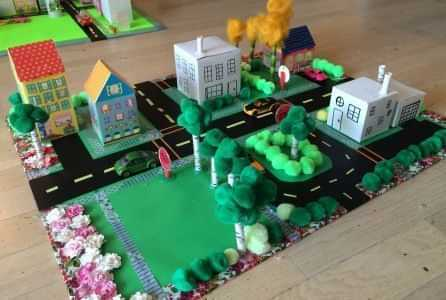
\includegraphics[width=\textwidth]{modelo.jpg}
    \caption{Modelo}
  \end{minipage}
\end{figure}

\end{frame}

\vspace{5mm}

\section{Análise Espectral}

\begin{frame}{Espectro de modelo ARMA}

\vspace{5mm}

Com a compreensão de modelos ARMA como o processamento linear de ruído branco
o a expressão para o espectro desses sinais é direta:

\vspace{5mm}

\begin{equation}\label{eq:arma_spectrum}
     S_{ARMA}(\omega) = \frac{\sigma^2 |1 + \sum_{k=1}^{q} b_k e^{-j\omega k}|^2}{2\pi|1 + \sum_{k=1}^{p} a_k e^{-j\omega k}|^2}
\end{equation}

\end{frame}

\begin{frame}{Raízes Unitárias}

A presença de raízes unitárias é facilmente compreendida sob a visão discutida.

\begin{figure}[H]
    \centering
    \includegraphics[scale=0.4]{../figures/arma_21.png}
    \caption{Sinal ARMA(2, 1) no domínio do tempo.}
    \label{fig:arma_21}
\end{figure}


\end{frame}

\begin{frame}{Raízes Unitárias}


\begin{figure}[H]
    \centering
    \includegraphics[scale=0.4]{../figures/arma_21_pzp.png}
    \caption{Diagrama de polos e zeros de ARMA(2, 1).}
\end{figure}


\end{frame}

\begin{frame}{Raízes Unitárias}


\begin{figure}[H]
    \centering
    \includegraphics[scale=0.4]{../figures/arma_21_diff_pzp.png}
    \caption{Diagrama de polos e zeros de ARMA(2, 1) diferenciado.}
\end{figure}


\end{frame}

\begin{frame}{Raízes Unitárias}


\begin{figure}[H]
    \centering
    \includegraphics[scale=0.4]{../figures/arma_21_diff.png}
    \caption{Sinal ARMA(2, 1) diferenciado visualizado no tempo.}
\end{figure}


\end{frame}

\begin{frame}{Raízes Unitárias}


\begin{figure}[H]
    \centering
    \includegraphics[scale=0.4]{../figures/arma_21_integrated_pzp.png}
    \caption{Diagrama de polos e zeros de ARMA(2, 1) integrado.}
\end{figure}


\end{frame}

\begin{frame}{Raízes Unitárias}


\begin{figure}[H]
    \centering
    \includegraphics[scale=0.4]{../figures/arma_21_integrated.png}
    \caption{Sinal ARMA(2, 1) integrado visualizado no tempo.}
\end{figure}


\end{frame}

\section{Aplicação}

\end{document}
